

\section{Введение}


\subsection{Цель работы}

Цель данной лабораторной работы заключается в изучении методов многократных прямых измерений физических величин, а также в освоении процедур обработки полученных данных для повышения их точности и достоверности. Для достижения поставленной цели необходимо выполнить серию измерений одной и той же физической величины, обработать полученные результаты с помощью статистических методов и оценить погрешности измерений.

Методы исследования включают использование стандартных измерительных приборов, математическое моделирование процессов, а также статистическую обработку данных с применением соответствующих формул для оценки погрешностей и анализа результатов.


\subsection{Решаемые задачи}
\begin{enumerate}
  \item Освоить методику использования измерительного прибора для
многократного прямого измерения физической величины.
  \item Выполнить простейшую статистическую обработку серии
результатов наблюдений при прямых измерениях.
\end{enumerate}

\section{Основная часть}

\subsection{Теоретическая часть}

В данной лабораторной работе используется метод многократных прямых измерений для регистрации данных с частотомера, который отображает временные диапазоны регистрации сигналов с генератора. Мы проводим серию измерений с целью определения средней величины, отклонений и оценки погрешностей, связанных с приборами.


Формула относительной погрешности прибора $\delta T$:
\begin{equation}
  \delta T = \pm (0,05 + 0,05  \frac{T_{\text{к}}}{T_{\text{х}}})\%
\end{equation}

Формула для нахождения среднего арифметического $\overline{T}$:
\begin{equation}
  \overline{T} = \frac{\sum_{i=1}^{n} T_i}{n}
\end{equation}
где $n$ - количество результатов отдельных наблюдений, $T_i$ - результат измерения отдельного наблюдения.

Вычисление погрешности прибора $\Delta T_{\text{приб}}$ определяется следующей формулой:
\begin{equation}
  \Delta T_{\text{приб}} = \frac{\delta T *\overline{T}}{100\%}
\end{equation}
Среднеквадратичное отклонение $\sigma$:
\begin{equation}
  \sigma \approx \sqrt{\frac{1}{n-1} \sum_{i = 1}^{n} (T_i -\overline{T}^2)}
\end{equation}
Средняя квадратичная погрешность среднего $\Delta T$:
\begin{equation}
  \Delta T = \sigma_{\overline{T}} \approx \frac{\sigma}{\sqrt{n}}
\end{equation}

\subsection{Эксперимент}
От генератора сигналов Г5-2А на частотомер Ч3-32 подается последовательность
трапецеидальных импульсов, диапозоны которых были заданы $0-10^6$ мс для грубой шкалы и $0-10^4$ мс для точной шкалы.
Задаваемое импульсы многократно измерялись цифровым частотомером. Все данные в ходе эксперимента записывались в протокол наблюдения.

\begin{figure}[H]
\centering
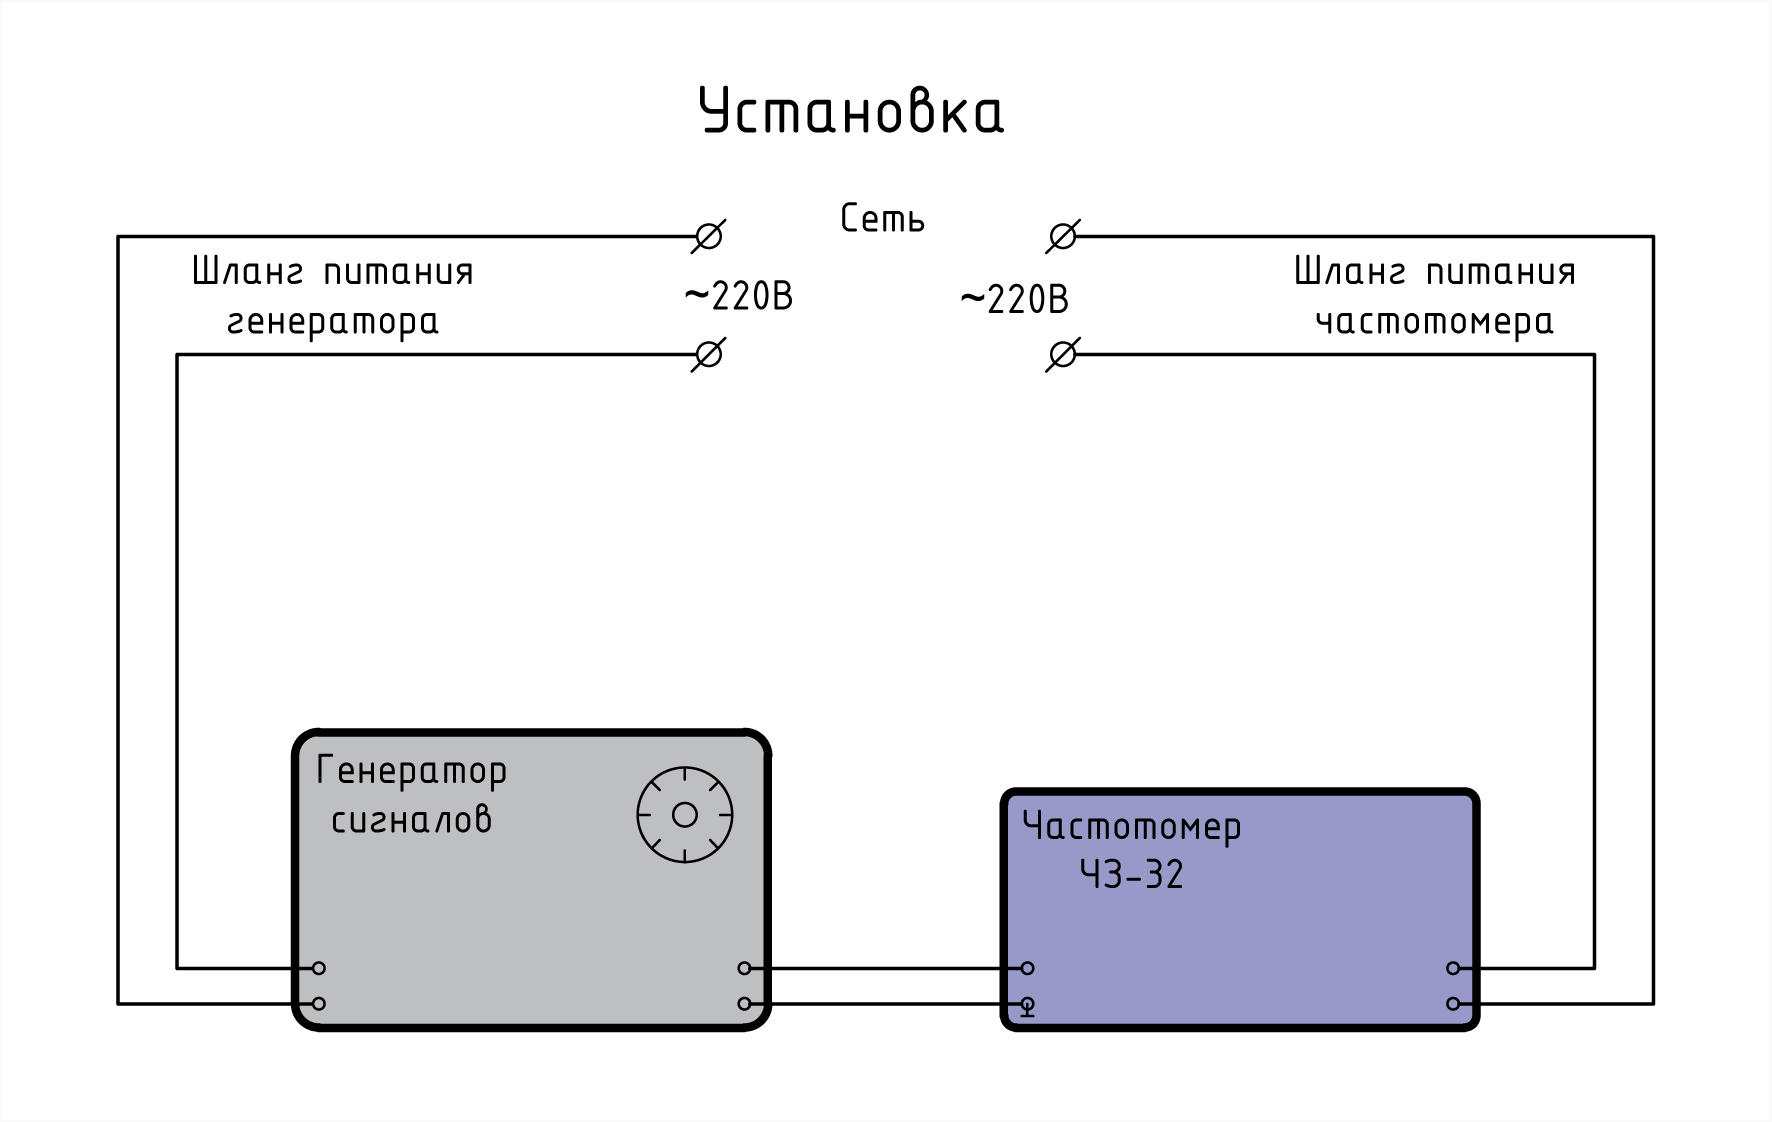
\includegraphics[width=0.6\textwidth]{Schema.png}
\caption{Схема установки}
\label{fig:sketch}
\end{figure}

\begin{figure}[H]
\centering
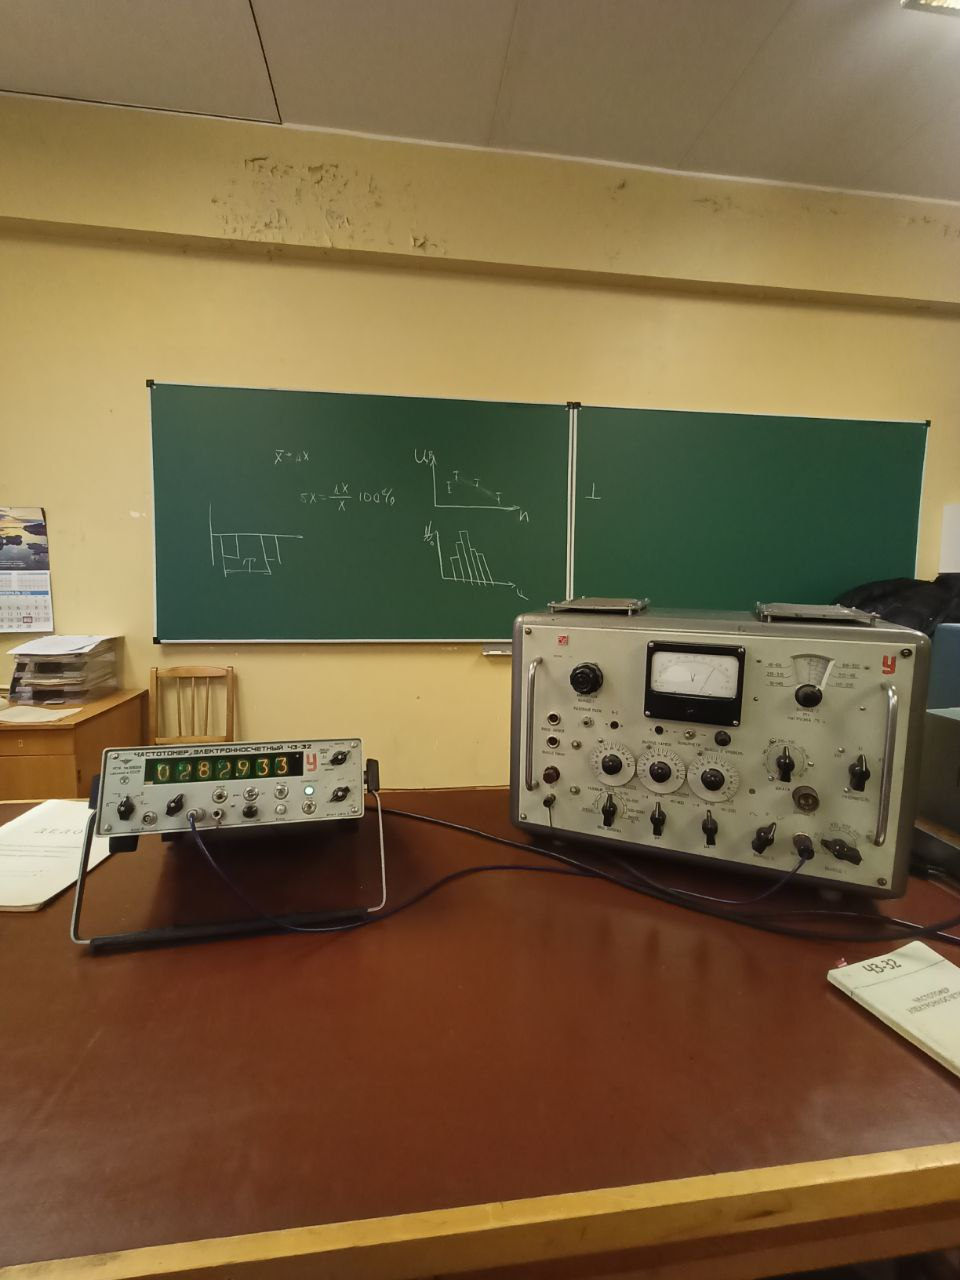
\includegraphics[width=0.6\textwidth]{Device.png}
\caption{Фотография установки}
\label{fig:device}
\end{figure}


\subsection{Обработка данных и обсуждение результатов}
Для написания программы, вычисляющей все требуемые данные, используется язык C++; среда разработки - Visual Studio.
Код полностью расположен в репозитории на GitHub.


\subsubsection{Исходный код} 

Программа выполняет обработку данных, считанных из файлов с точными и грубыми измерениями. Вначале открывается файл с точными значениями, и все строки с числами считываются в вектор. После этого вычисляется среднее значение для этих данных, и это значение используется для вычисления отклонений от среднего для каждого числа в векторе. Далее программа рассчитывает квадрат этих отклонений, что соответствует стандартному отклонению, и выводит результаты.

После вычисления стандартного отклонения программа вычисляет среднюю погрешность прибора, используя заранее определённые параметры. Далее, с использованием функции, которая рассчитывает погрешности на основе значений времени и других параметров, программа выводит погрешности для каждого значения.

Аналогично проводятся измерения и для грубых, и для точных значений.

\begin{lstlisting}[label=listing1, caption=Вычисление среднего,]
/ Функции для вычислений
double avarage(const vector<double>& data)
{
    double sum = 0.0;
    for (double u : data)
    {
        sum += u;
    }
    return sum / data.size();
}

vector<double> standartDeviation(vector<double>& randDevAr)
{
    vector<double> standAr;
    for (int i = 0; i < randDevAr.size(); i++)
    {
        double t = randDevAr[i];
        standAr.push_back(t * t);
    }
    return standAr;
}

vector<double> randomDeviation(const vector<double>& data, double avarage)
{
    vector<double> randDevAr;
    for (int i = 0; i < data.size(); i++)
    {
        randDevAr.push_back(data[i] - avarage);
    }

    return randDevAr;
}

vector<double> calculateDeltaT(const vector<double>& Tx_values, double gamma0, double T0, double T_avg)
{
    vector<double> deltaT_results;
    for (double Tx : Tx_values)
    {
        double gamma_T = gamma0 + (T0 / Tx);
        deltaT_results.push_back(gamma_T * T_avg);
    }
    return deltaT_results;
}


    // Вычисление среднего значения
    double mean = avarage(values);
    cout << "Среднее значение (точные): " << mean << endl;

    // Вычисление отклонений от среднего для каждого значения
    cout << "Отклонения от среднего: " << endl;

    vector<double> ar1 = randomDeviation(values, mean);

    for (int i = 0; i < ar1.size(); i++)
    {
        cout << ar1[i] << "\n";
    }
    cout << endl;

    // Вычисление стандартного отклонения

    cout << "Стандартное отклонение: " << endl;

    vector<double> ar2 = standartDeviation(ar1);
    for (int i = 0; i < ar2.size(); i++)
    {
        cout << ar2[i] << "\n";
    }
    cout << endl;

    // Вычисление средней погрешности прибора
    cout << "Средняя погрешность прибора: " << endl;

    cout << (gamma0 + (T0 / mean)) * mean << "\n";
    cout << endl;

    // Вычисление погрешностей
    cout << "Погрешности (точные): " << endl;

    vector<double> delta_T1 = calculateDeltaT(values, gamma0, T0, mean);
    for (int i = 0; i < delta_T1.size(); i++)
    {
        cout << delta_T1[i] << "\n";
    }
    cout << endl;
}

\end{lstlisting}

\clearpage
\subsubsection{Таблицы}
\begin{center}
\begin{table}[h!]
\centering
\caption{Результаты грубых измерений}
\label{tabl:1}
\begin{tabular}{|c|c|c|c|c|}
\hline
\begin{minipage}{7mm}
    № п.п. 
\end{minipage}&
\begin{minipage}{5cm}
    Диапазон показаний использованной шкалы прибора
\end{minipage} &
\begin{minipage}{5cm}
    Результаты отдельных наблюдений ($T_i$)
\end{minipage} &
\begin{minipage}{5cm}
    Погрешность прибора на данной шкале ($\Delta T_{\text{приб}}$)
\end{minipage}\\
\hline
{}&мс&мс&мс\\
\hline
1 &	$0-10^6$ &	282.7 & 0.000240974 \\
2 &	$0-10^6$ &	281.7 & 0.000241329 \\
3 &	$0-10^6$ &	282.5 & 0.000241045 \\
4 &	$0-10^6$ &	282.0 & 0.000241222 \\
5 & $0-10^6$ &	282.0 & 0.000241222 \\
6 & $0-10^6$ &	282.9 & 0.000240904 \\
7 & $0-10^6$ &	281.8 & 0.000241293 \\
8 & $0-10^6$ &	282.6 & 0.00024101 \\
9 & $0-10^6$ &	282.1 & 0.000241187 \\
10& $0-10^6$ &	282.3 & 0.000241116 \\
\hline
\end{tabular}
\end{table}
\end{center}

\begin{center}
\begin{table}[h!]
\centering
\caption{Результаты точных измерений}
\label{tabl:2}
\begin{tabular}{|c|c|c|c|c|}
\hline
\begin{minipage}{7mm}
    № п.п. 
\end{minipage}&
\begin{minipage}{5cm}
    Результаты отдельных наблюдений (Ti)
\end{minipage} &
\begin{minipage}{5cm}
    Случайные отклонения от среднего $d_i = T_i - \overline{T}$
\end{minipage} &
\begin{minipage}{5cm}
     $d_i^2 = (T_i - \overline{T})^2$
\end{minipage}\\
\hline
{}&мс&мс&мс\\
\hline
1 &	282.926  &	0.4746 & 0.225245 \\
2 &	281.803  &	-0.6484	& 0.420423 \\
3 &	282.582  &	0.1306	& 0.0170564 \\
4 &	282.693  &	0.2416 & 0.0583706 \\
5 & 281.794  &	-0.6574 & 0.432175 \\
6 & 282.524  &	0.0726 & 0.00527076 \\
7 & 282.220  &	-0.2314 & 0.053546 \\
8 & 282.786  &	0.3346 & 0.111957 \\
9 & 281.807  &	-0.6444 & 0.415251 \\
10& 282.256  &	-0.1954 & 0.0381812 \\
11& 282.973  &	0.5216 & 0.272067 \\
12& 282.224  &	-0.2074 & 0.0430148 \\
13& 281.997  &	-0.4544 & 0.206479 \\
14& 282.622  &	0.1706 & 0.0291044 \\
15& 282.770  &	0.3186 & 0.101506 \\
\hline
\end{tabular}
\end{table}
\end{center}

\begin{center}
\begin{table}[h!]
\centering
\caption{Результаты точных измерений}
\label{tabl:2}
\begin{tabular}{|c|c|c|c|c|}
\hline
\begin{minipage}{7mm}
    № п.п. 
\end{minipage}&
\begin{minipage}{5cm}
    Результаты отдельных наблюдений (Ti)
\end{minipage} &
\begin{minipage}{5cm}
    Случайные отклонения от среднего $d_i = T_i - \overline{T}$
\end{minipage} &
\begin{minipage}{5cm}
     $d_i^2 = (T_i - \overline{T})^2$
\end{minipage}\\
\hline
{}&мс&мс&мс\\
\hline
16& 283.136  &	0.6846 & 0.468677 \\
17& 282.735  &	0.2836 & 0.080429 \\
18& 282.340  &	-0.1114 & 0.01241 \\
19& 282.339  &	-0.1124 & 0.0126338 \\
20& 282.128  &	-0.3234 & 0.104588 \\
21& 282.258  &	-0.1934 & 0.0374036 \\
22& 282.489  &	0.0376 & 0.00141376 \\
23& 282.505  &	0.0536 & 0.00287296 \\
24& 282.958  &	0.5066 & 0.256644 \\
25& 282.638  &	0.1866 & 0.0348196 \\
26& 282.345  &	-0.1064 & 0.11321 \\
27& 281.898  &	-0.5534 & 0.306252 \\
28& 282.345  &	-0.1064 & 0.011321 \\
29& 282.684  &	0.2326 & 0.0541028 \\
30& 283.159  &	0.7076 & 0.500698 \\
31& 282.816  &	0.3646 & 0.132933 \\
32& 281.950  &	-0.5014 & 0.251402 \\
33& 282.197  &	-0.2544 & 0.0647194 \\
34& 282.422  &	-0.0294 & 0.00086436 \\
35& 282.430  &	-0.0214 & 0.00045796 \\
36& 282.642  &	0.1906 & 0.0363284 \\
37& 282.971  &	0.5196 & 0.269984 \\
38& 282.580  &	0.1286 & 0.016538 \\
39& 282.115  &	-0.3364 & 0.113165 \\
40& 281.863  &	-0.5884 & 0.346215 \\
41& 282.017  &	-0.4344 & 0.188703 \\
42& 282.424  &	-0.0274 & 0.00075076 \\
43& 282.675  &	0.2236 & 0.049997 \\
44& 283.157  &	0.7056 & 0.497871 \\
45& 282.442  &	-0.0094 & 0.00008836 \\
46& 281.895  &	-0.5564 & 0.309581 \\
47& 281.993  &	-0.4584 & 0.210131 \\
48& 282.236  &	-0.2154 & 0.0463972 \\
49& 282.728  &	0.2766 & 0.0765076 \\
50& 283.063  &	0.6116 & 0.374055 \\
\hline
\end{tabular}
\end{table}
\end{center}

\begin{table}[h!]
\centering
\caption{Таблица для построения гистограммы и кривой распределения}
\label{tabl:1}
\begin{tabular}{|c|c|c|c|c|}
\hline
\begin{minipage}{7mm}
    № интервала 
\end{minipage}&
\begin{minipage}{5cm}
    Границы интервалов (ширина интервала $\Delta h = 0.1814$)
\end{minipage} & 
\begin{minipage}{5cm}
    Число случаев ($\Delta n$), когда результат наблюдения попадает в данный интервал
\end{minipage} & 
\begin{minipage}{5cm}
    Доля (часть) полного числа результатов, попадающих в данный интервал ($\delta n = \frac{\Delta n}{n}$)
\end{minipage}\\
\hline
1 &  281.345 & 1 &  0.02\\
2 &  281.526 & 2 & 0.04 \\
3 &  281.708 & 3 & 0.06 \\
4 &  281.890 & 4 & 0.08 \\
5 & 282.071 & 9 & 0.18 \\
6 & 282.252 & 7 & 0.14 \\
7 & 282.433 & 8 & 0.16 \\
8 & 282.615 & 8 & 0.16 \\
9 & 282.796 & 5 & 0.10 \\
10& 282.977 & 3 &  0.06 \\
\hline
\end{tabular}
\end{table}

\subsubsection{Графики}


\begin{figure}[ht!]
\centering
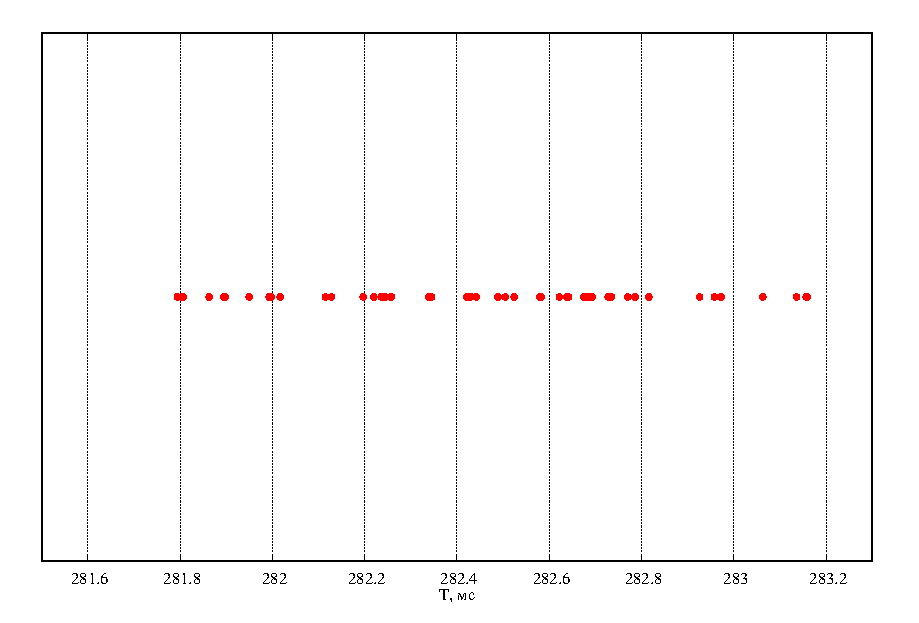
\includegraphics[width=0.8\textwidth]{time_i.eps}
\caption{Зависимость измерений от времени}
\label{fig:plot}
\end{figure}

\begin{figure}[ht!]
\centering
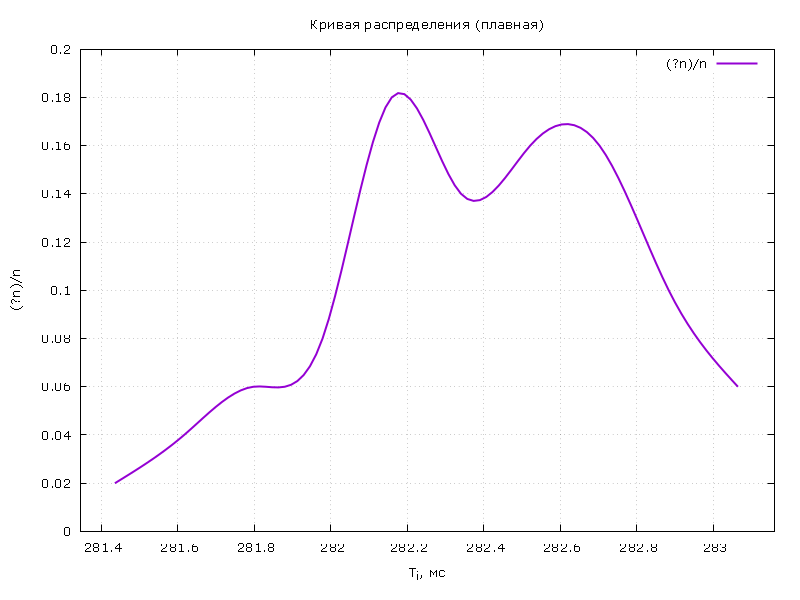
\includegraphics[width=0.8\textwidth]{smooth_distribution_curve.png}
\caption{Плотность распределения}
\label{fig:plot}
\end{figure}

\begin{figure}[ht!]
\centering
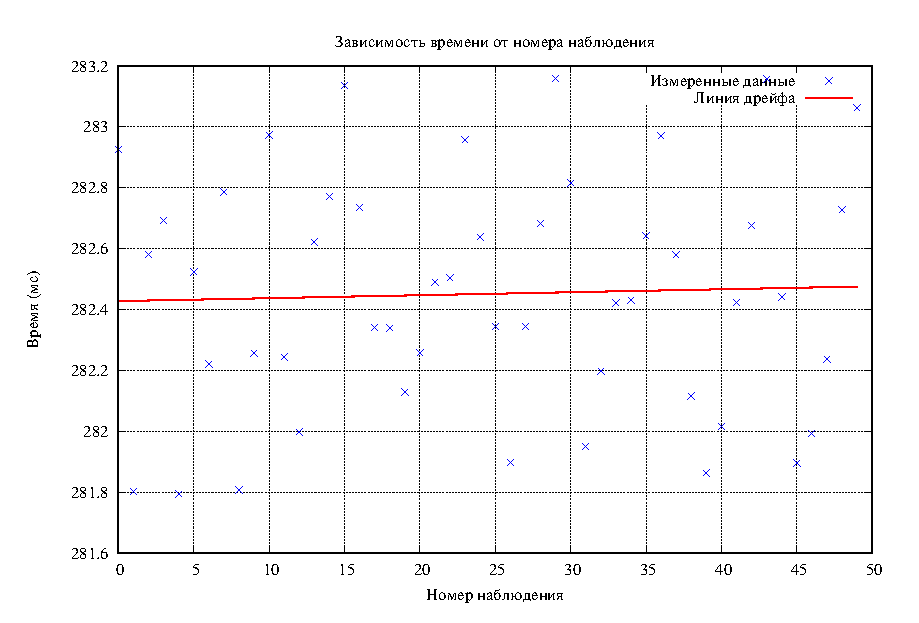
\includegraphics[width=0.8\textwidth]{time_drife.eps}
\caption{Зависимость измерений от времени}
\label{fig:plot}
\end{figure}

\begin{figure}[ht!]
\centering
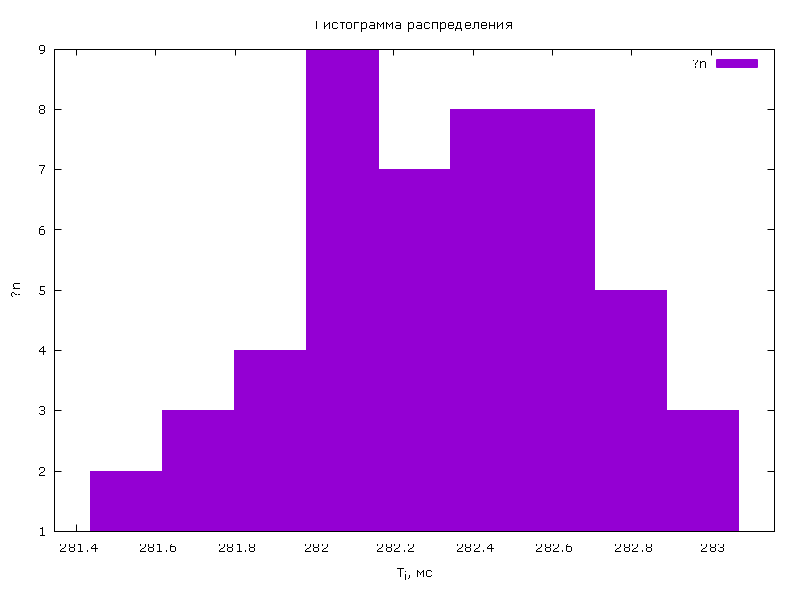
\includegraphics[width=0.8\textwidth]{histogram_rounded.png}
\caption{Гистограмма}
\label{fig:plot}
\end{figure}

\clearpage
\section{Выводы}
В ходе выполнения работы я приобрела навыки использования измерительных приборов для многократных прямых измерений физических величин. 
Научилась работать с частотомером и разобралась в методах статистической обработки результатов, включая расчет дисперсии и среднеквадратичного отклонения. Попробовала работать в среде gnuplot для реализации графиков.. 

% Список литературы
% Для отчёта он не обязателен
\begin{thebibliography}{9}

%ссылка на репозиторий с исходныим кодом отчета и всех расчетных программ обязательна 
\bibitem{repo}
\url{https://github.com/st106773/Workshop1.git} 

\end{thebibliography}


